\section{Development environment and simulation}
\label{sec:devenv}
During the process of developing the application, it became necessary to be able to continuously deploy and test the latest version without having to depend on flying the physical vehicle but instead relying on the simulation of the system inside the computer that was at the same time running the developed software.
This configuration has the twofold advantage of reducing the development time on the one hand, since there is no need to be concerned with the interactions between the different hardware components and the results can be visualized immediately on the computer screen, and on the other hand increasing the safety of the process by only running on the vehicle software that has already been tested to an acceptable point.

Simulators allow PX4 flight code to control a computer-modeled vehicle in a simulated "world" that can be interacted with in the same ways as with a real vehicle, using QGroundControl, an offboard API or a radio controller/gamepad. 
PX4 supports two different simulation modes: software-in-the-loop (\gls{sitl}), where the flight stack runs on an external computer, and hardware-in-the-loop (\gls{hitl}), where it uses a simulation firmware on an actual flight controller board.
Communication into and out of the flight stack uses the MAVLink protocol mentioned in section \ref{subsec:mavlink},
which allows exchanging of messages defined within XML files between drones, ground control stations, and other MAVLink systems \cite{mavlink}.
When the firmware is simulated, a MAVLink server is always started as part of the running software to enable communication with the simulator program and any other offboard entry point that could be present.


\begin{figure}
  \centering
  
\includegraphics[width=\textwidth,keepaspectratio]{img/px4_simulator_messages.png}
  \caption{Mavlink messages exchanged between the simulator and the flight stack during simulation.}
  \source{Adapted from \citetitle{px4-guide} \cite{px4-guide}.}
  \label{fig:simulator-msgs}
\end{figure}

In both SITL and HITL modes, the simulation works according to the feedback loop shown in figure~\ref{fig:simulator-msgs}. 
The simulator generates the input from the sensors based on its internal world representation and sends it through Mavlink messages to the flight stack running on the same computer using the \gls{udp} transport protocol,
which in turn generates response actuator controls that are fed back into the simulator in the same way to affect the vehicle's position, velocity, and attitude in the simulated world.
Simulated communications employ MAVLink messages specific to the mode in use and are not precisely the same as those used during non-simulated flight.

There are many options for simulators supported by PX4, like Gazebo, a powerful 3D simulation environment for Linux systems that is particularly suited for testing object avoidance and is commonly used with ROS, or AirSim (\ref{subsec:airsim}). This more resource-intensive cross-platform simulator leverages the Unreal Engine, typically used for game development and animation, to provide physically and visually realistic simulations.
For this project, AirSim was chosen because of previous experience with Unreal Engine as well as for the easy availability of visual packages to test computer vision features and its native support for running on Windows machines, which is the operating system running on the computer where the tests will take place.
AirSim offers as well a Python library called \texttt{airlib} (\footnote{\url{https://pypi.org/project/airsim/}}) that can be used to retrieve images taken from a simulated camera from the perspective of the drone in the simulation world.
This feature will be necessary when testing the person-recognition utilities used in the program.

\begin{figure}
  \centering
  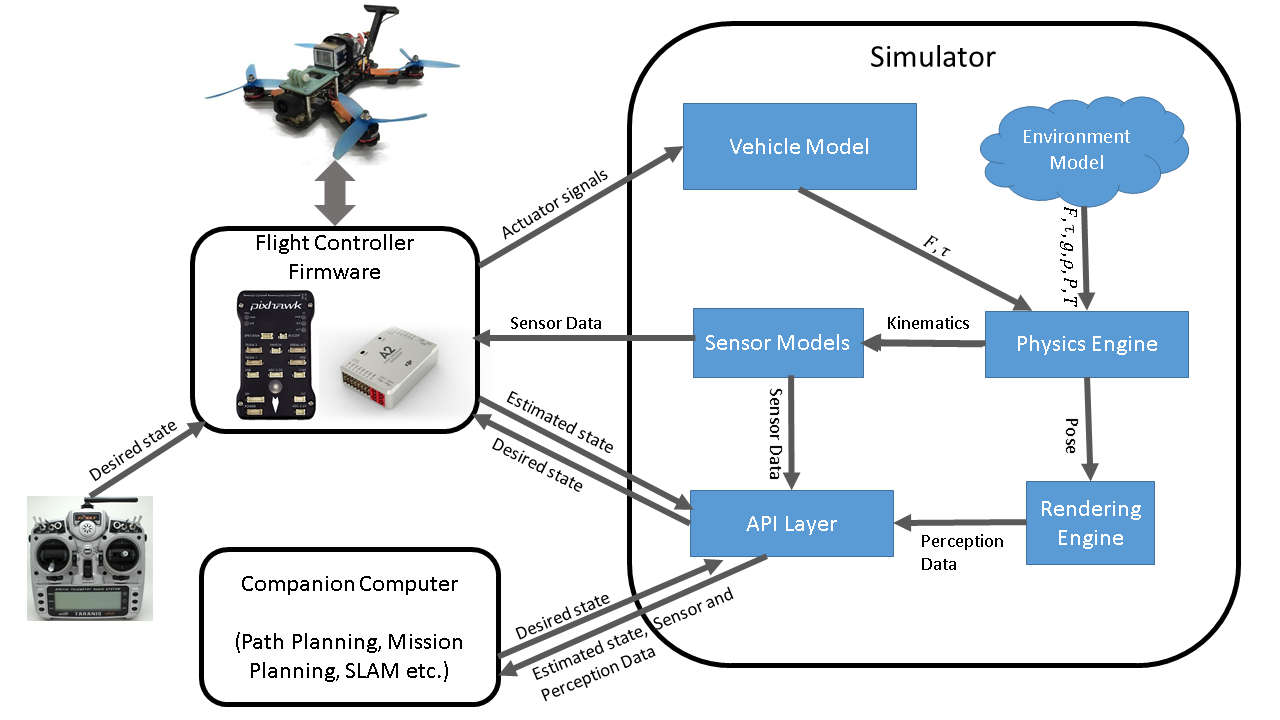
\includegraphics[width=\textwidth,keepaspectratio]{img/airsim-overview.png}
  \caption{High-level overview of how different components interact in the AirSim simulator.}
  \source{Adapted from \citetitle{airsim-paper} \cite{airsim-paper}.}
  \label{fig:airsim-overview}
\end{figure}
\todo[inline]{Final polish: export all boards again from Miro without watermarks}

A high-level overview of the simulator architecture and the way different components interact with each other can be seen in figure~\ref{fig:airsim-overview}. 
The API layer present in the Figure inside the simulator environment refers to AirSim's own airlib library, which exposes with high-level functionality to send control commands to the flight controller directly.
However, in order to share the same control code when simulating flight and in real flight without and not depend on the simulator system, the control commands are sent using the official MavSDK API instead, which allows communication of estimated state, desired state and sensor data directly between the flight controller firmware and the companion computer.

In order to run software-in-the-loop simulation, the PX4 firmware needs to be built from the source code on the Linux platform where it is going to run.
The build system then sets up all the necessary ports for the Mavlink communication and starts a local instance of the NuttX operating system that runs on the actual flight board.
\begin{figure}
  \centering
  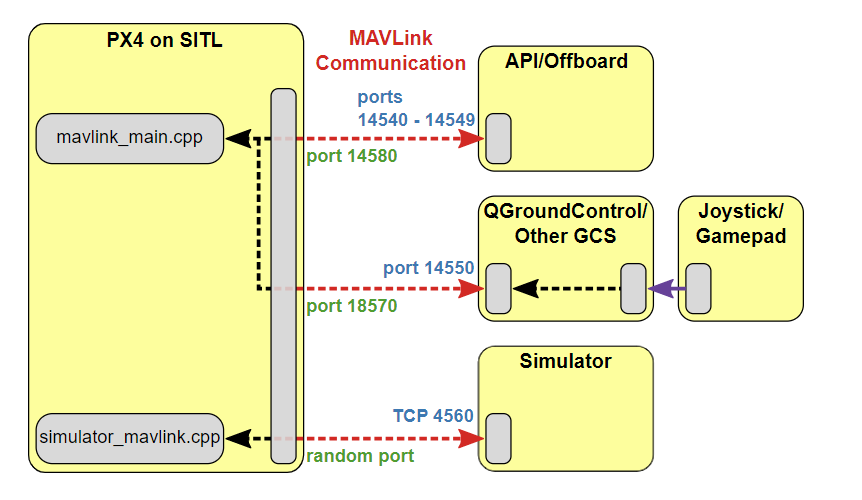
\includegraphics[width=\textwidth,keepaspectratio]{img/px4-ports.png}
  \caption{Network diagram between the different components that interconnect during software-in-the-loop simulation.}
  \source{Adapted from \citetitle{px4-guide} \cite{px4-guide}.}
  \label{fig:px4-ports}
\end{figure}
Figure~\ref{fig:px4-ports} shows how the different parts of the system communicate with each other inside a SITL simulation.
PX4 uses commonly established UDP ports for MAVLink communication with ground control stations (e.g. QGroundControl), offboard APIs (e.g. MAVSDK, MAVROS) and simulator APIs (e.g. AirSim, Gazebo).
External developer application like Dronecontrol use an offboard API, in this case MAVSDK, and therefore listen to PX4's remote UDP port 14540.
All ports in the range 14540-14549 can be used to connect offboard API, for example in the case of controlling multiple vehicles at the same time.
PX4's remote UDP Port 14550 is used for communication with ground control stations, which are expected to listen for connections on this port (QGroundControl listens to this port by default).
PX4 uses a simulation-specific module to connect to the simulator's local TCP port 4560. 
Simulators then exchange information with PX4 using the Simulator MAVLink API shown in Figure~\ref{fig:simulator-msgs}. 
PX4 on SITL and the simulator can run on either the same computer or different computers on the same network.

Since the purpose of using AirSim as a simulator is to run it on a Windows computer and the PX4 software-in-the-loop stack runs on Linux, it is necessary to run a virtualized Linux OS in parallel on the Windows computer and setup a local network so that the simulator and the flight controller firmware can communicate with each other.
The PX4 development team officially supports running the SITL flight stack in Windows through the Windows Subsystem for Linux (WSL2)\footnote{\url{https://docs.microsoft.com/en-us/windows/wsl/about}}, which allows users to install and run their Ubuntu Development Environment on Windows as if it was running it on a Linux computer.
The Windows Subsystem for Linux lets developers run a GNU/Linux environment (including most command-line tools, utilities, and applications) directly on Windows, unmodified, without the overhead of a traditional virtual machine or dualboot setup.
The full steps needed for to configure the system are detailed in Section~\ref{sec:test2}.

\begin{figure}
  \centering
  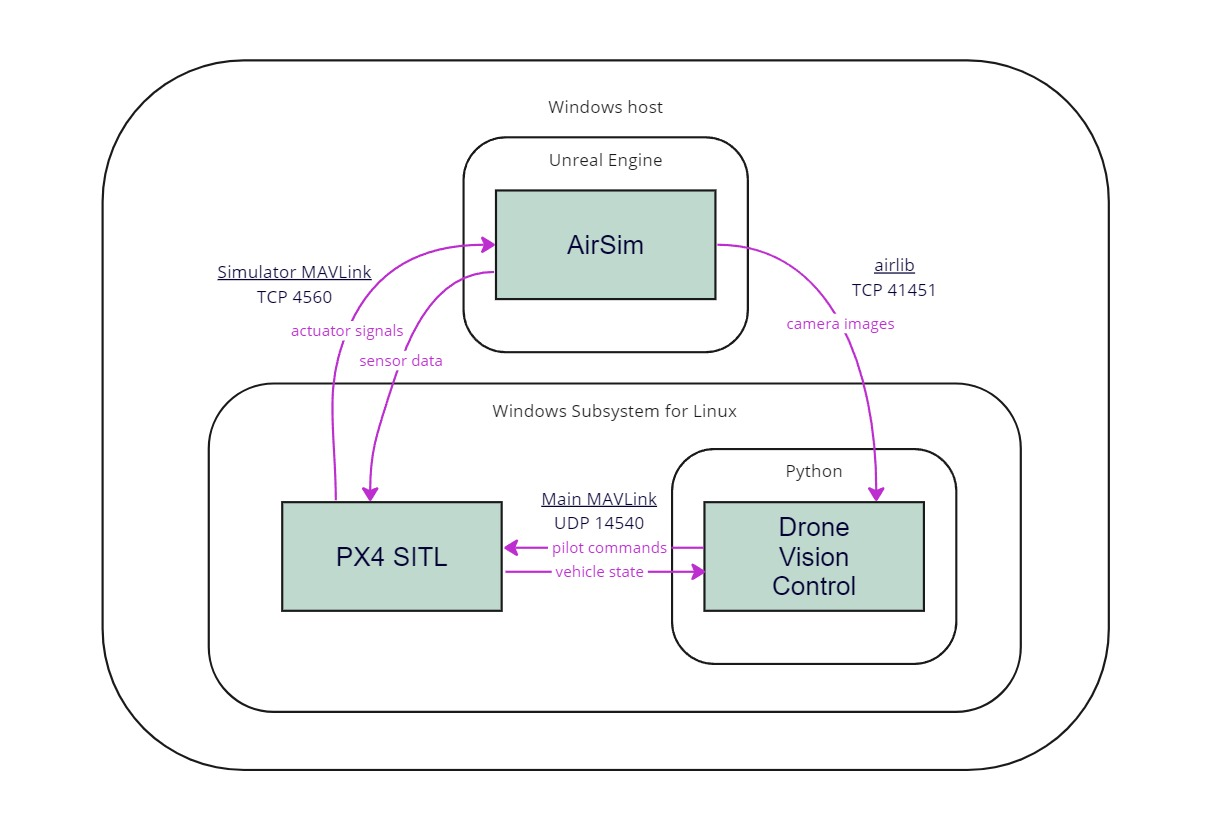
\includegraphics[width=\textwidth,keepaspectratio]{img/sitl-connections.jpg}
  \caption{Connection diagram of how the three systems interact with each other during SITL simulation.}\label{fig:sitl-connections}
\end{figure}
The whole set of connections established in the software-in-the-loop simulation is shown in Figure~\ref{fig:sitl-connections} at the transport layer level. The two systems that run inside the virtualized Linux system through WSL (the simulated flight stack and the dronecontrol program) connect through the localhost network on the UDP port defined by PX4 for Offboard APIs and each of them connects in turn to the AirSim simulator through the virtual Local Area Network established by the Windows Subsystem for Linux to the host Windows computer.
The PX4 flight stack on SITL mode connects to the simulator using the TCP port 4560, as defined by PX4 on Figure~\ref{fig:px4-ports}, and dronecontrol connects through the AirSim library which uses by default a TCP connection on port 41451.

In the case of hardware-in-the-loop simulation, the main difference with SITL is that the flight stack firmware runs on a physical flight board using a special configuration.
In HITL all motors/actuators are blocked, but internal software is fully operational.
This configuration adds an additional separated operating system and to make this mode of testing simpler, since the WSL environment is no longer needed to run the flight stack, it is possible to move the execution of the Python module to Windows.
This eliminates the need to add further configuration to allow the external flight controller to communicate with the internal WSL network, which is by default only accessible by its Windows host computer.
Moreover, now that PX4 runs on a separate piece of hardware, it is necessary to establish two separate physical connections to the Windows computer, so that both the simulator and the Python app can communicate through their own channel to the flight controller, either wired, to the microUSB port or an unused telemetry port on the flight controller, or wireless through a telemetry radio.

\begin{figure}
  \centering
  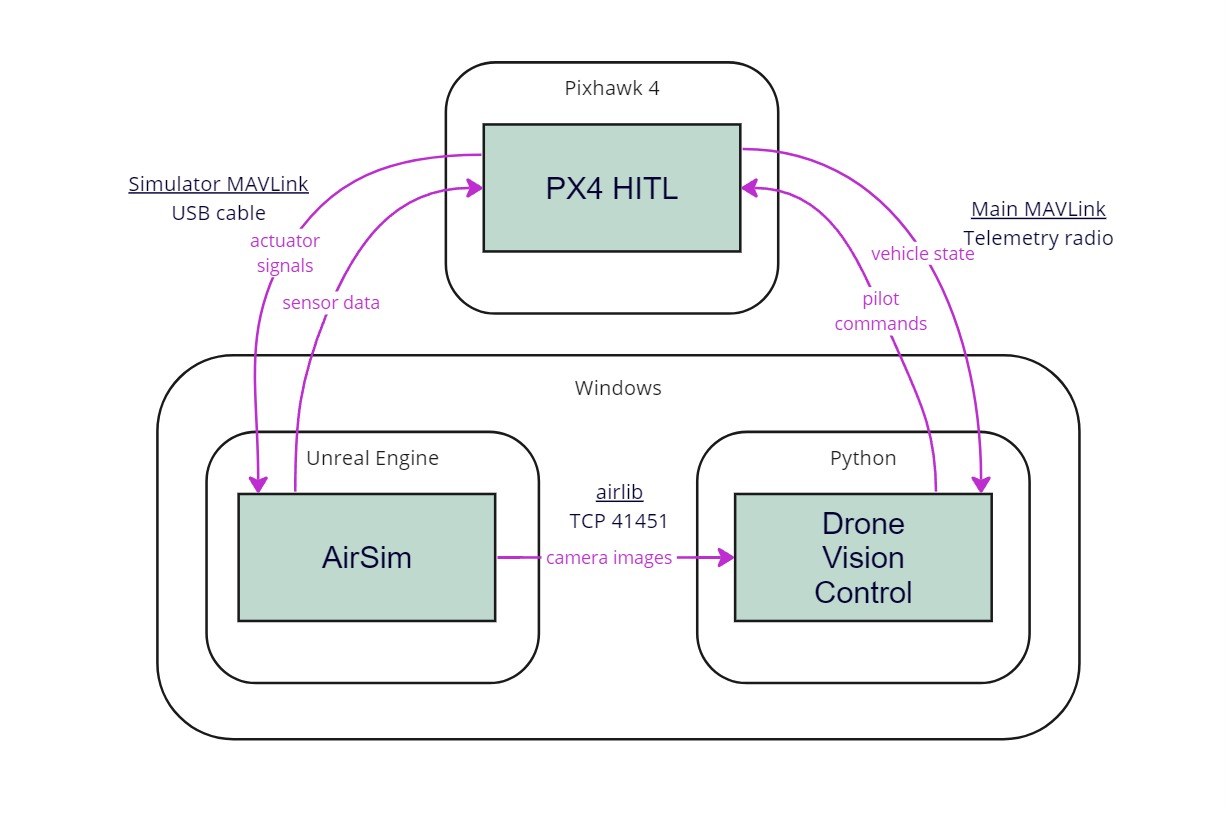
\includegraphics[width=\textwidth,keepaspectratio]{img/hitl-connections.jpg}
  \caption{Connection diagram of how the three systems interact with each other during HITL simulation.}\label{fig:hitl-connections}
\end{figure}

Figure~\ref{fig:hitl-connections} shows the chosen connections to execute tests in HITL mode.
The Windows machine runs both AirSim and the Python interpreter, which communicate through the \texttt{localhost} network using TCP.
The board running PX4 connects to the simulator through a USB to microUSB cable, which is setup to work with a baudrate of 115200, and to the developed program through a telemetry radio running at a baudrate of 57600, both attached to USB ports on the Windows computer accessible through their COM address.

\subsubsection{AirSim testing environment}

Unreal Engine is a complex computer graphics generation program.
It works by creating environments where components like 3D models, cameras, and lighting can be added.
AirSim is a plugin made for this engine by Microsoft, and although it also has a release for the other main game engine in the market, Unity, it is experimental and limited in features.
The documentation contains all the necessary steps to get Unreal Engine and AirSim running on a Windows, Linux, or macOS operating system. 
However, it works best on Windows \cite{build-airsim}.
The source code for the AirSim project includes a built-in Unreal environment that can be used to run tests and contains several 3D shapes like block and spheres, as well as a default quadcopter to act as the control vehicle.
It is also possible to create custom Unreal environments and run AirSim inside them by adding the built plugin to the project and a custom vehicle.

The environment used in this project for testing the Dronecontrol application is derived from the built-in AirSim environment.
It contains the default quadcopter vehicle, which includes several virtual cameras in order to be able to retrieve images from the vehicle's point of view in the simulated world, and a few of the preset blocks with a green color to give a better contrast to the camera.
The main addition to the environment is the 3D model of a human figure, to be used for testing the pose detection and tracking mechanisms of the computer vision solution.
The model is part of a free asset library of human models made by Renderpeople \cite{render-people} obtained in the Unreal Marketplace.
An image of the testing environment can be seen in figure \ref{fig:unreal-env}.


\begin{figure}
  \centering
  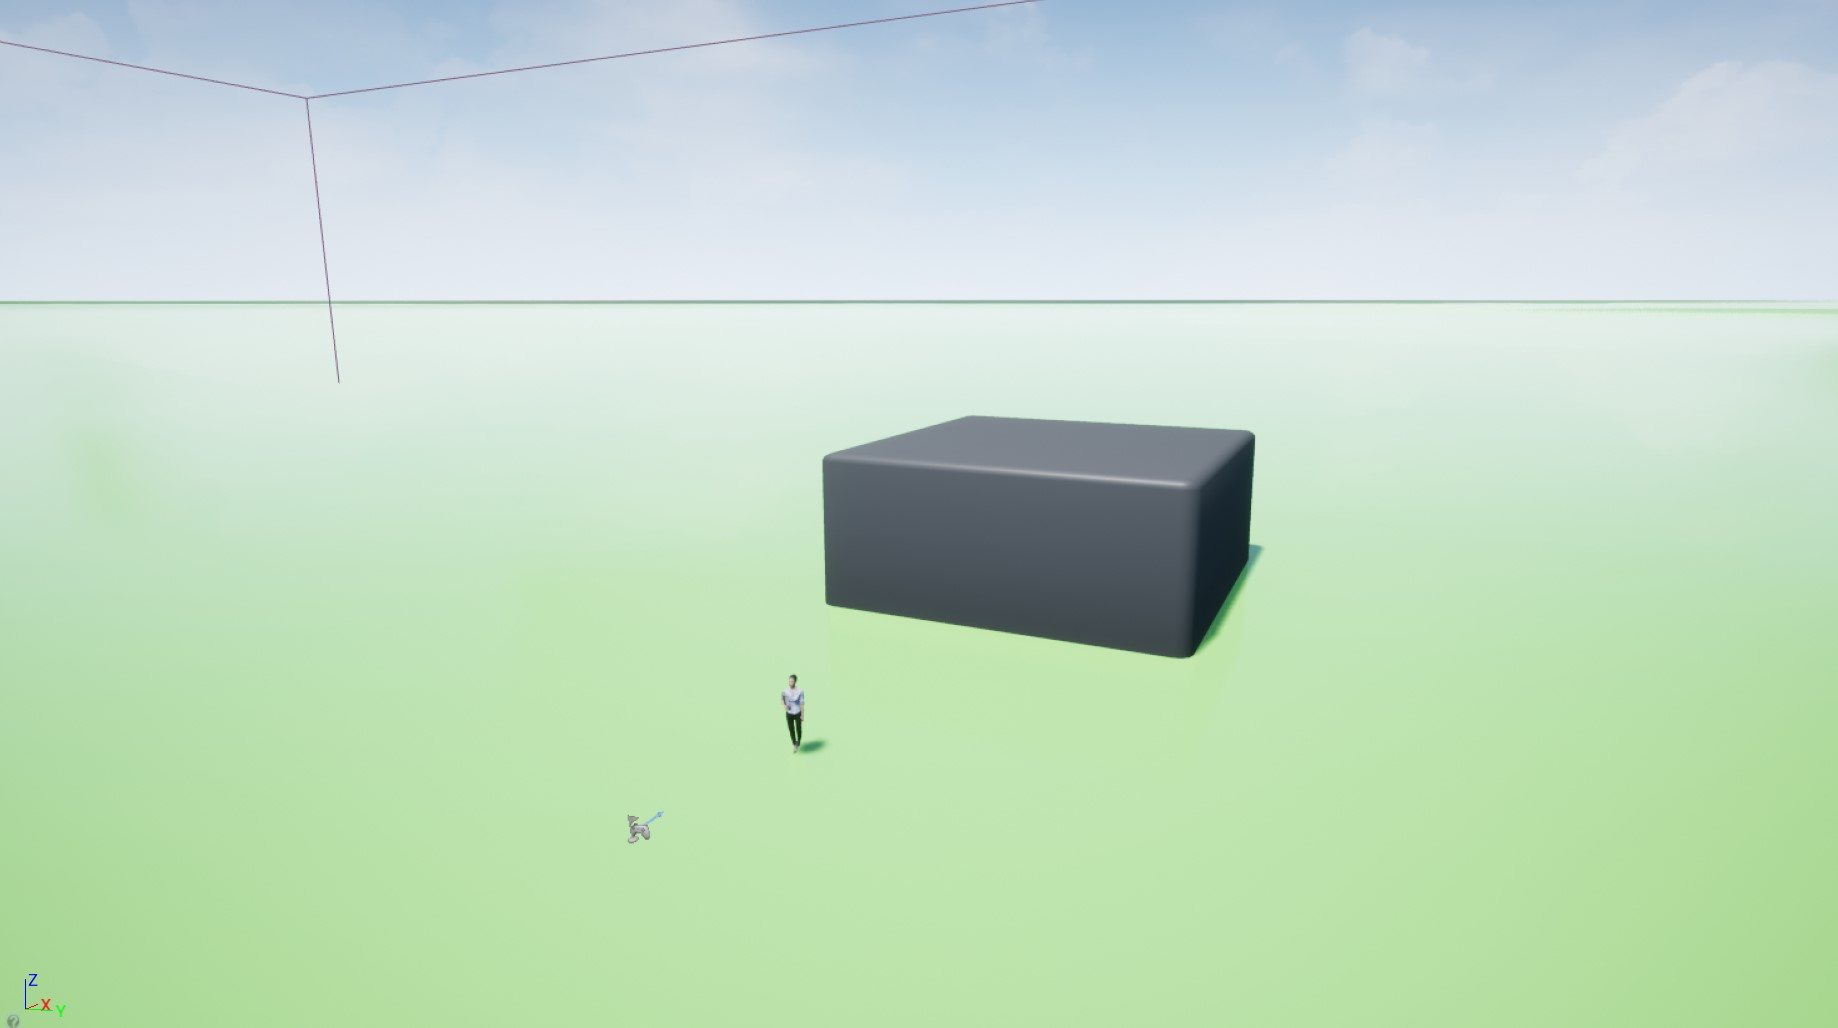
\includegraphics[width=\textwidth,keepaspectratio]{img/unreal-env.jpg}
  \caption{Screenshot from the Unreal Engine environment used for testing the computer vision solutions.}
  \label{fig:unreal-env}
\end{figure}


AirSim is compatible both with SITL and HITL simulation.
However, it is necessary to set it up to work with an external PX4 flight controller instead of AirSim's own internal \texttt{SimpleFlight}.
Appendix \ref{app:airsim-config} shows all the required settings for configuring these modes in AirSim.
To run the simulator in Windows and the flight controller in WSL, the IP of the Windows host in the \texttt{vEthernet (WSL)} network needs to be provided in the AirSim settings.
This process is detailed further in the AirSim documentation \cite{airsim-doc-wsl}.
In brief, first the Unreal project with AirSim has to be set into play mode and then the PX4 SITL flight controller built and run to attach to an already running simulator.
Inside the project in WSL, the flight controller can be run for AirSim by using the provided shortcut script \footnote{\url{https://github.com/l-gonz/tfg-giaa-dronecontrol/blob/main/simulator.sh}}:
\begin{minted}{bash}
sh simulator.sh --airsim
\end{minted}
Once both the simulator and the flight controller are connected, an RC controller or QGroundControl can be used to control the vehicle, and other offboard applications like Dronecontrol can be attached to send any desired MAVLink commands.
